\documentclass[12pt,twoside]{article}
\usepackage[a4paper,includefoot,margin=2.54cm]{geometry}

% MATH %
\usepackage{amsmath}


% LISTS %
\usepackage{enumitem}

% remove top lists separation
\setlist{noitemsep,topsep=-\parskip}


% URL HIGHLIGHTING %
\usepackage[hyphens,spaces,obeyspaces]{url} % for formatting urls
\usepackage[hidelinks, unicode,
						colorlinks = true,
						linkcolor = black,
						urlcolor  = blue,
						citecolor = black,
						anchorcolor = black]{hyperref}


% CODE %
\usepackage{minted} % highlight code with Pygments

\setminted{linenos,                     % number lines
           breaklines,                  % break lines that exceed the line width
           autogobble,                  % remove common leading whitespace
					 baselinestretch=1,           % line stretch
					 frame=lines,                 % add frame (top and bottom lines)
					 framesep=6pt,			 					% text and frame separation
					 fontsize=\footnotesize}      % decrease size to fit line widths

% reduce spacing in code examples
\usepackage{etoolbox}
\BeforeBeginEnvironment{minted}{\vspace{-\parskip}}
\setlength\partopsep{-\topsep}


% GRAPHICS
\usepackage{float} % the [H] floats option
\usepackage{graphicx}


% FONT AND ENCODING %
\usepackage[T1]{fontenc} % font encoding
\usepackage{fontspec}    % font selector
\setmainfont{CMU Serif}  % main font


% DATETIME FORMATTING %
\usepackage[UKenglish]{isodate}
\cleanlookdateon % 10 October 2018


% TEXT FORMATTING %
\usepackage{titlesec}
\usepackage{setspace}

% define subsubsubsection as parahraph
\titleformat{\paragraph}{\bfseries\normalsize}{\theparagraph}{1em}{}
\setcounter{secnumdepth}{4}
\setcounter{tocdepth}{4}

\setlength\itemindent{0pt}
\setlength\parskip{9pt}
\setlength\parindent{0pt}

\titlespacing{\section}      {0pt}{0pt}{6pt}
\titlespacing{\subsection}   {0pt}{0pt}{4pt}
\titlespacing{\subsubsection}{0pt}{0pt}{2pt}
\titlespacing{\paragraph}    {0pt}{0pt}{0pt}

% create the command subsubsubsection
\let\subsubsubsection\paragraph

% increase the baseline stretch for readability
\renewcommand{\baselinestretch}{1.15} % baseline stretch is 1.15

\widowpenalty10000 % prevent widows
\clubpenalty10000  % prevent orphans

% define KaTeX logo
\makeatletter
\DeclareRobustCommand{\KaTeX}{%
  K\kern -.19em
  {\sbox \z@ T\vbox to\ht \z@ {\hbox{%
  \check@mathfonts
  \fontsize\sf@size\z@
  \selectfont A}%
  \vss}%
}\kern -.15em
\TeX}
\makeatother

% ---------------------------------------------------------------------------- %

\begin{document}

% suppress page numbering
\pagenumbering{gobble}

% prevent text overflow
\sloppy

\begin{titlepage}
	\begin{center}
    \vspace*{2cm}
		\Huge \textbf{Robotics Simplified}\\
		\normalsize \vspace{0.5cm}
		Generated \today.
	\end{center}
\end{titlepage}

\cleardoublepage

% resume page numbering
\pagenumbering{arabic}
\setcounter{page}{1}%

\tableofcontents

\cleardoublepage


\section{Preface}


Although you don't need to know any robotics before reading through this website, there are some things that can make your learning experience much more pleasant.


\subsection{Math}
To understand the math on this website, it is best to understand basic algebra, trigonometry, geometry. None of the math should exceed high-school level and if it does, there will be links to resources to explain them. \textbf{Even if math weren't your strong suit and you skipped all of the equations, you'd still learn a lot!}


\subsection{Programming}
Understand basic concepts of programming will definitely come in handy before reading through the project. There are lots of great resources for learning programming:
\begin{itemize}
\item Reddit's \href{https://www.reddit.com/r/learnprogramming/}{r/learnprogramming} forum.
\item \href{https://www.codecademy.com/}{Codeacademy} and their \href{https://www.codecademy.com/learn/learn-python-3}{Learn Python 3} course.
\item \href{https://projecteuler.net/}{Project Euler} for practicing programming on fun math-based problems.
\end{itemize}\vspace{\parskip}

Knowing syntax of Python would also be helpful, since all of the code examples discussed in the project are written in Python. If you don't know much about Python, but already know how to program in a different language, \href{http://histo.ucsf.edu/BMS270/diveintopython3-r802.pdf}{Dive into Python 3} is a great place to start.

\textbf{If you don't know anything about programming but are interested in learning robotics anyway, you can still read through the chapters} -- the code is included mainly to showcase possible implementations of the discussed concepts.


\subsection{Libraries and Classes}
Throughout the project, there will be a lot of made-up classes like \texttt{Motor}, \texttt{Joystick} and \texttt{Gyro}. They are only used as placeholders for real classes that you would (likely) have, if you were implementing some of the concepts covered on this website on a platform of your choosing.


\subsection{About comments}
There are a LOT of comments in the examples of code that you are about to see. Way, way more than there should be. I agree that this is considered bad practice for practical purposes and that if you are a relative beginner, you shouldn't write code in a similar fashion.

However, since the purpose of the code on this website is educational and not to serve as a part of a codebase, I would argue that it is fine to use them to such extent.





\section{Running the Code}


The code on this website has been tested on a VEX EDR robot programmed in Python using \href{https://www.robotmesh.com/}{RobotMesh}. If you want to try out the code yourself, doing the same would be the easiest way -- all you'd have to do is substitute the made-up classes and methods for real ones from the VEX library and run the code.

\begin{figure}[H]
\centering
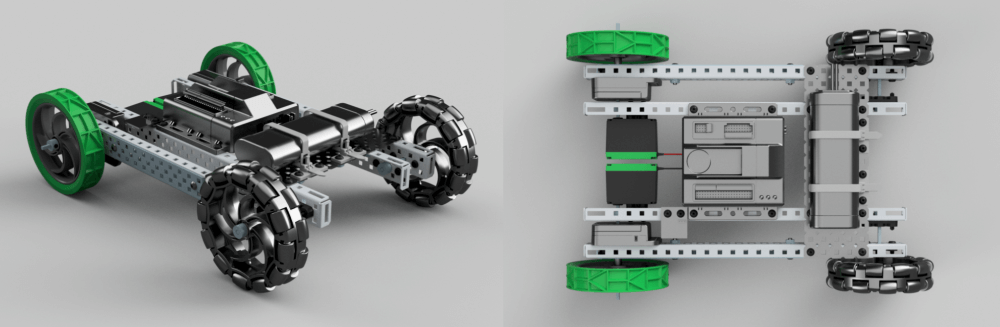
\includegraphics[width=0.8\textwidth]{../assets/images/robot.png}
\caption{Robot Model}
\end{figure}

You can download the robot model in the STEP format from \href{https://grabcad.com/library/vex-edr-robot-1}{this link}, if you're interested!





\section{Drivetrain Control}




\begin{figure}[H]
\centering
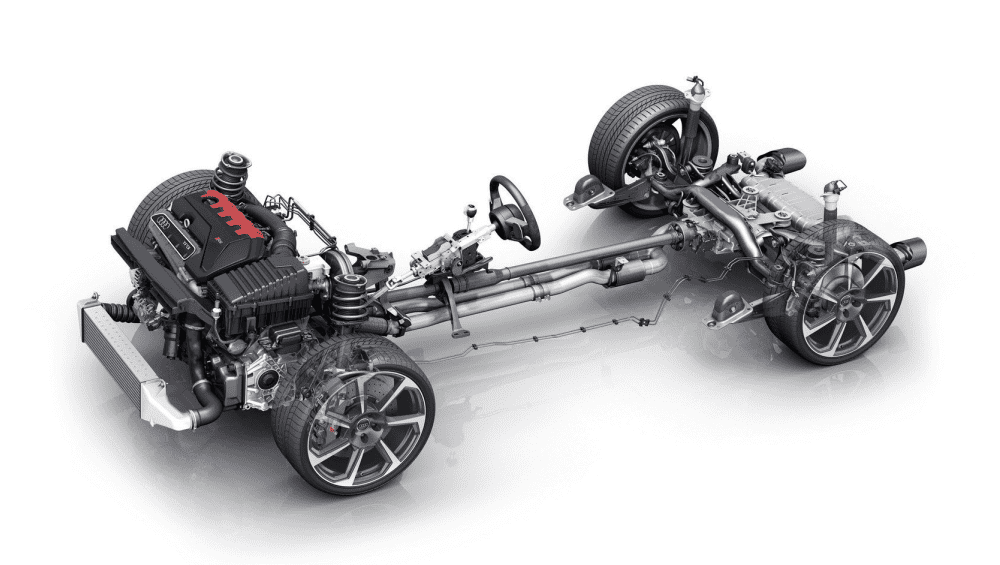
\includegraphics[width=0.8\textwidth]{../assets/images/drivetrain-control/drivetrain.png}
\caption{Drivetrain}
\end{figure}


The drivetrain of a vehicle is a group of components that deliver power to the driving wheels, hold them together and allow them to move. Some of the \href{http://www.simbotics.org/resources/mobility/drivetrain-selection}{most popular ones} are:
\begin{itemize}
\item \textbf{tank drive} -- left and right side motors are driven independently -- like a \textit{tank}
\item \textbf{mecanum drive} -- similar to tank drive, but uses \href{http://www.wcproducts.net/wheels-hubs/mecanum-wheels}{mecanum wheels}, each of which is driven independently -- allows for more maneuverability
\item \textbf{swerve drive} -- each wheel can rotate vertically around its axis -- the robot can drive and rotate in any direction
\end{itemize}\vspace{\parskip}

For the purpose of this guide, however, we will only be discussing some of the most frequently used drivetrains, and the methods to operate them.




\subsection{Tank drive}
Tank drive is a method of controlling the motors of a \textit{tank drive drivetrain} using two axes of a controller, where each of the axes operate motors on one side of the robot (see image below, or \href{https://www.youtube.com/watch?v=vK2CGj8gAWc}{this video}).

\begin{figure}[H]
\centering
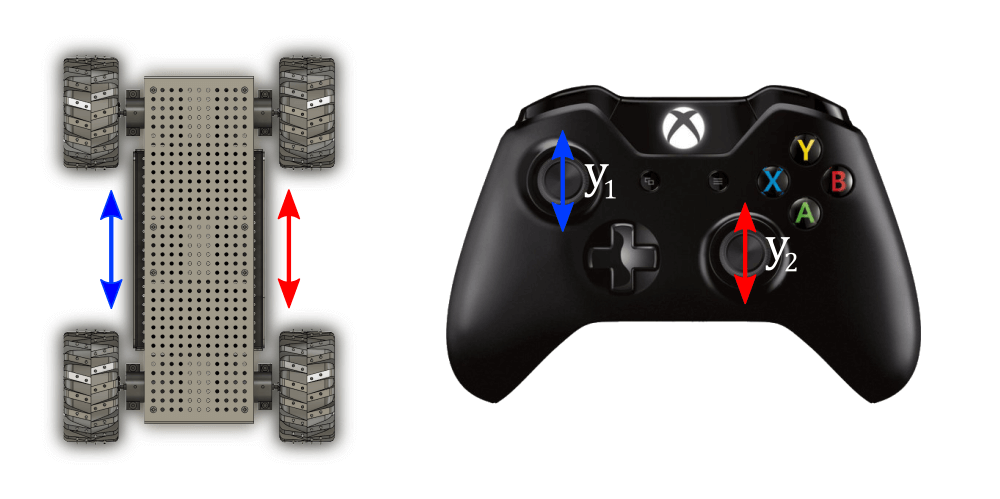
\includegraphics[width=0.8\textwidth]{../assets/images/drivetrain-control/tank-drive.png}
\caption{Tank Drive}
\end{figure}


\subsubsection{Implementation}
Suppose that we have objects of the \texttt{Motor} class that set the speed of the motors that take values from -1 to 1. We also have a \texttt{Joystick} object that returns the values of the $y_1$ and $y_2$ axes.

Implementing tank drive is quite straightforward: set the left motor to the $y_1$ axis value, and the right motor to the $y_2$ axis value:

\begin{minted}{python}
def tank_drive(l_motor_speed, r_motor_speed, left_motor, right_motor):
    """Drives the robot using tank drive."""
    left_motor(l_motor_speed)
    right_motor(r_motor_speed)
\end{minted}



\subsubsection{Examples}
The following example demonstrates, how to make the robot drive using tank drive controlled by a joystick.

\begin{minted}{python}
# initialize objects that control robot components
left_motor = Motor(1)
right_motor = Motor(2)
joystick = Joystick()

# repeatedly set motors to the values of the axes
while True:
    # get axis values
    y1 = joystick.get_y1()
    y2 = joystick.get_y2()

    # drive the robot using tank drive
    tank_drive(y1, y2, left_motor, right_motor)
\end{minted}



\subsubsection{Closing remarks}
Tank drive is a very basic and easy way to control the robot. When it comes to FRC, it is a method used frequently for its simplicity, and because it is easier for some drivers to control the robot this way, compared to the other discussed methods.




\subsection{Arcade drive}
Arcade drive is a method of controlling the motors of a \textit{tank drive drivetrain} using two axes of a controller, where one of the axes controls the speed of the robot, and the other the steering of the robot.

\begin{figure}[H]
\centering
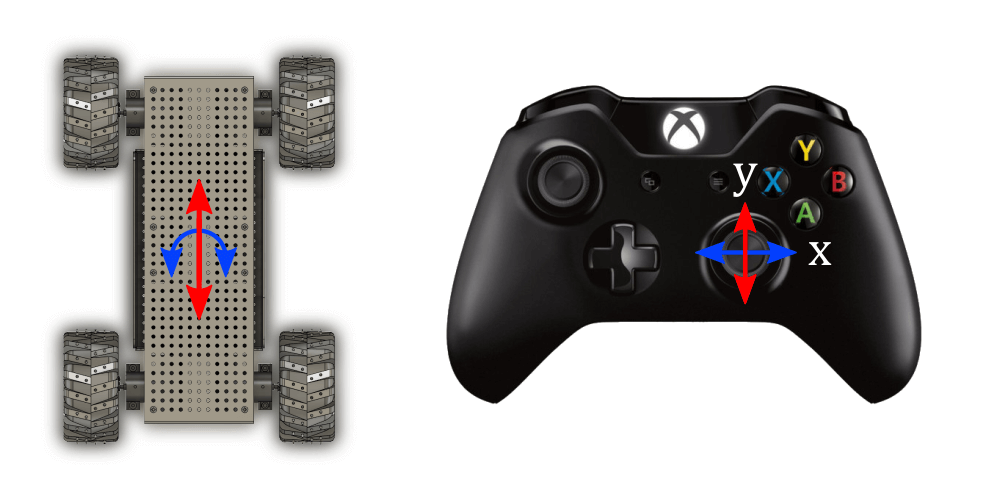
\includegraphics[width=0.8\textwidth]{../assets/images/drivetrain-control/arcade-drive.png}
\caption{Arcade Drive}
\end{figure}


\subsubsection{Deriving the equations}
The equations used in the implementation are derived using \href{https://en.wikipedia.org/wiki/Linear_interpolation}{linear interpolation}. This allows us to transition from one coordinate to the other in a linear fashion, which provides a pleasant driving experience.

I won't show the derivation here, since it isn't too exciting (if you're interested, it can be found in \href{https://www.chiefdelphi.com/t/paper-arcade-drive/168720}{this post} on Chief Delphi), but rather an illustration to help you understand the derivation more intuitively.

\begin{figure}[H]
\centering
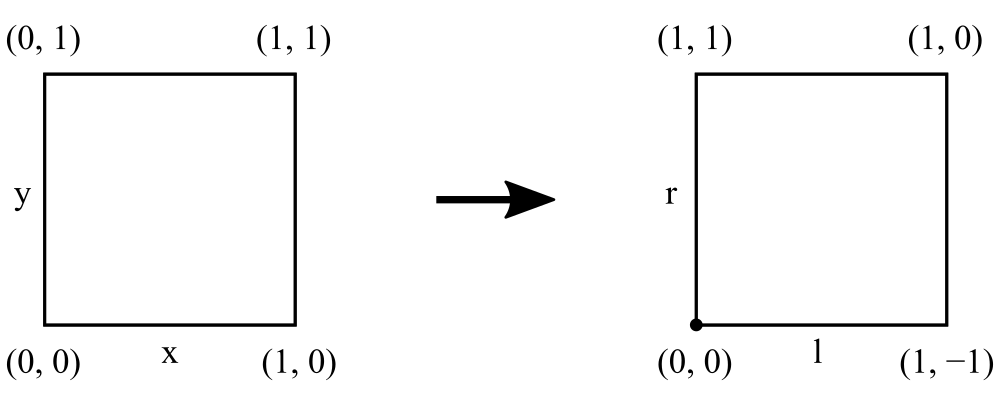
\includegraphics[width=0.8\textwidth]{../assets/images/drivetrain-control/arcade-drive-illustration.png}
\caption{Arcade Drive Illustration}
\end{figure}

What we want is to transform our $x$ and $y$ coordinates to the speeds of the motor. To do this, let's focus on the values we would \textit{like} to be getting in the 1st quadrant. The left rectangle in the illustration represents the joystick values (in the 1st quadrant) and right one the speeds of the left and right motor (in the 1st quadrant). I would suggest you see the visualization at the end of the article, it demonstrates this nicely.

The speeds of the left motor $l$ are $1$ in all of the corners (besides the origin). Using $x, y$, we can achieve the same values by saying that $l$ is the bigger of the two... $l = \text{max}(x, y)$.

As for the right motor $r$, As the $x$ and $y$ change their values, $r$ goes from $1$ (top left) to $-1$ (bottom right). We can model the same values using difference... $r = y - x$.

A similar observation can be made about the other quadrants. This is mostly to show that you can think about the derivations more intuitively (since this particular one it isn't too complicated).


\subsubsection{Implementation}
\begin{minted}{python}
def arcade_drive(rotate, drive, left_motor, right_motor):
    """Drives the robot using arcade drive."""
    # variables to determine the quadrants
    maximum = max(abs(drive), abs(rotate))
    total, difference = drive + rotate, drive - rotate

    # set speed according to the quadrant that the values are in
    if drive >= 0:
        if rotate >= 0:  # I quadrant
            left_motor(maximum)
            right_motor(difference)
        else:            # II quadrant
            left_motor(total)
            right_motor(maximum)
    else:
        if rotate >= 0:  # IV quadrant
            left_motor(total)
            right_motor(-maximum)
        else:            # III quadrant
            left_motor(-maximum)
            right_motor(difference)
\end{minted}



\subsubsection{Examples}
The following example demonstrates, how to make the robot drive using arcade drive controlled by a joystick.

\begin{minted}{python}
# initialize objects that control robot components
left_motor = Motor(1)
right_motor = Motor(2)
joystick = Joystick()

# repeatedly set motors to the values of the axes
while True:
    # get axis values
    x = joystick.get_y1()
    y = joystick.get_y2()

    # drive the robot using adcade drive
    arcade_drive(x, y, left_motor, right_motor)
\end{minted}



\subsubsection{Closing remarks}
If you are interested in reading more about this topic, I would suggest looking at \href{https://www.chiefdelphi.com/media/papers/2661}{this thread on Chief Delphi}, where I learned most of the information about the theory behind arcade drive.




\section{Motor controllers}





It's nice to be able to drive the robot around using a joystick, but it would sometimes be more useful if the robot could drive \textbf{autonomously} (independently). This is where controllers come in.

A controller is a box that takes in information about the robot and a goal that we want the robot to achieve (like drive a certain distance / turn a certain angle) and, when asked, returns values it thinks the robot should set its motors to, to achieve that goal.

The are lots of various controllers to choose from that differ in many ways, such as:
\begin{itemize}
\item \textbf{Accuracy} -- how accurate is the controller in getting the robot where it needs to be? How error-prone is it to unexpected situations (a bump on the road, motor malfunction,...).
\item \textbf{Input} -- what of information does the controller needs to function properly (and accurately)? Does the information have to be real-time?
\item \textbf{Complexity} -- how difficult is it to implement/configure said controller? How computationally intensive it is?
\end{itemize}\vspace{\parskip}

There is a whole field of study called \href{https://en.wikipedia.org/wiki/Control_theory}{control theory} that examines controllers much more comprehensively than we can in a few short articles. That's why we're only going to talk about a select few.




\subsection{Sample Controller Class}
Although each of the controllers will operate quite differently, they will all have (nearly) identical functions, that will allow us to use them interchangeably, without breaking the rest of the code.

\begin{minted}{python}
class SampleControllerClass:
    """Description of the class."""

    def __init__(self, ...):
        """Creates a controller object."""
        pass

    def set_goal(self, goal):
        """Sets the goal of the controller."""
        pass

    def get_value(self):
        """Returns the current controller value"""
        pass
\end{minted}


\texttt{\_\_init\_\_} is called when we want to create a controller object. In the actual controller implementations, "\texttt{...}" will be replaced by the parameters that the controller takes.

\texttt{set\_goal} is called to set the controller's goal, where goal has to be a number. Note that we will need to call this function before trying to call \texttt{get\_value}, or things will break. This makes sense, because the controller can't really help you to reach the goal if you haven't specified it yet.

\texttt{get\_value} will return the value that the controller thinks we should set the motors to, to achieve our goal. \textbf{All controllers will return values between (and including) -1 and 1,} since it's more convenient to do math on numbers in that range.

All of this will make more sense as we go through each of the controllers.




\subsection{Dead reckoning}
One of the simplest ways of controlling the robot autonomously is using \href{https://en.wikipedia.org/wiki/Dead_reckoning}{dead reckoning}.

It uses one of the first equations you learned in physics: $time = distance / speed$. We use it to calculate, how long it takes something to travel a certain distance based on its average speed.

Let's look at an example: say our robot drives an average of $s = 2.5 \frac{m}{s}$. We want it to drive a distance of $d = 10m$. To calculate, how long it will take the robot, all you have to do is divide distance by speed: $t = d/s = 10/2.5 = 4s$.

This is exactly what dead reckoning does -- it calculates the time it will take the robot to drive the distance to the goal. When asked, returns 1 if that amount of time hasn't elapsed yet and 0 if it has.


\subsubsection{Implementation}
There are two things that the controller needs: the average speed of the robot and a way to measure how much time had passed.

\begin{minted}{python}
class DeadReckoning:
    """A class implementing a dead reckoning controller."""

    def __init__(self, speed, get_current_time):
        """Takes the average speed and a function that returns current time."""
        self.get_current_time = get_current_time
        self.speed = speed

    def set_goal(self, goal):
        """Sets the goal of the controller (and also starts the controller)."""
        self.goal = goal
        self.start_time = self.get_current_time()

    def get_value(self):
        """Return the current value the controller is returning."""
        # at what time should we reach the destination (d=d_0 + s/v)
        arrival_time = self.start_time + (self.goal / self.speed)

        # return +-1 if we should have reached the destination and 0 if not
        if self.get_current_time() < arrival_time:
            return 1 if self.goal > 0 else -1
        else:
            return 0
\end{minted}


As we see, the parameters the \texttt{\_\_init\_\_} function is expecting to get are:
\begin{itemize}
\item \texttt{speed} -- the average speed of the robot.
\item \texttt{get\_current\_time} -- a function that returns the current time to measure, whether the calculated time had elapsed.
\end{itemize}\vspace{\parskip}


\subsubsection{Example}
\begin{minted}{python}
# initialize objects that control robot components
left_motor = Motor(1)
right_motor = Motor(2)

# create a controller object and set its goal
controller = DeadReckoning(2.5, get_current_time)
controller.set_goal(10)

while True:
    # get the controller value
    controller_value = controller.get_value()

    # drive the robot using tank drive controlled by the controller value
    tank_drive(controller_value, controller_value, left_motor, right_motor)
\end{minted}


This is an implementation of the problem proposed in the Introduction: make a robot drive 10 meters.

Notice how we used our previously implemented \texttt{tank\_drive} function to set both motors to drive forward. We could have written \texttt{left\_motor(controller\_value)} and \texttt{right\_motor(controller\_value)}, but this is a cleaner way of writing it.


\subsubsection{Closing remarks}
Although this is quite a simple controller to implement, you might realize that it is neither accurate nor practical. If the robot hits a bump on the road or slips on a banana peel, there is nothing it can do to correct the error, since it doesn't know where it is.

Another important thing to keep in mind when using this controller is that if you want to change how fast the robot is driving/turning, you will need to re-calculate the average speed of the robot, which is very tedious.

We'll be focusing on improving accuracy in the upcoming articles by incorporating real-time data from the robot into our controllers.




\subsection{Bang–bang}
Although our previous controller was quite easy to implement and use, there is no way for it to know whether it reached the target or not. It pretty much just turns the motors on for a while and hopes for the best.

\href{https://en.wikipedia.org/wiki/Bang\%E2\%80\%93bang_control}{Bang-bang} aims to fix this problem by using \href{https://en.wikipedia.org/wiki/Feedback}{feedback} from our robot. Feedback could be values from its \href{https://en.wikipedia.org/wiki/Encoder}{encoders} (to measure how far it has gone), \href{https://en.wikipedia.org/wiki/Gyroscope}{gyro} (to measure where it's heading), or really anything else that we wish to control. The important thing here is that the data is \textbf{real-time}. The robot continuously tells the controller what is happening, so the controller can act accordingly.

Bang-bang implements the very first idea that comes to mind when we have real-time data available. The controller will return 1 if we haven't passed the goal yet and 0 if we have.


\subsubsection{Implementation}
The only thing the Bang-bang controller needs is the feedback function returning information about the state of whatever we're trying to control.

\begin{minted}{python}
class Bangbang:
    """A class implementing a bang-bang controller."""

    def __init__(self, get_feedback_value):
        """Create the bang-bang controller object from the feedback function."""
        self.get_feedback_value = get_feedback_value

    def set_goal(self, goal):
        """Sets the goal of the bang-bang controller."""
        self.goal = goal

    def get_value(self):
        """Returns +1 or -1 (depending on the value of the goal) when the robot
        should be driving and 0 when it reaches the destination."""
        if self.goal > 0:
            if self.get_feedback_value() < self.goal:
                return 1    # goal not reached and is positive -> drive forward
        else:
            if self.get_feedback_value() > self.goal:
                return -1   # goal not reached and is negative -> drive backward

        # if it shouldn't be driving neither forward nor backward
        return 0
\end{minted}


\subsubsection{Examples}
To make the robot drive a distance using this controller, we need a new \texttt{Encoder} class to measure how far the robot has driven. The objects of this class return the average of the distance driven by the left wheel and by the right wheel.

\begin{minted}{python}
# initialize objects that control robot components
left_motor = Motor(1)
right_motor = Motor(2)
encoder = Encoder()

# create a controller object and set its goal
controller = Bangbang(encoder)
controller.set_goal(10)

while True:
    # get the controller value
    controller_value = controller.get_value()

    # drive the robot using tank drive controlled by the controller value
    tank_drive(controller_value, controller_value, left_motor, right_motor)
\end{minted}


Notice that pretty much nothing changed between this and the dead reckoning example. This is the main advantage of all of the controllers having the same functions -- we can use controller objects almost interchangeably, allowing us to easily try out and compare the accuracies of each of the controllers, without messing with the rest of our code.


\subsubsection{Closing remarks}
This is already markedly better than our previous dead reckoning approach, but it is still relatively inaccurate: the robot's inertia will make the robot drive a little extra distance when the controller tells it that it shouldn't be driving anymore, which means it will likely overshoot.

We could try to fix this by saying that it should start driving backward once it passed the goal, but the only thing you'd get is a robot that drives back and forth across the goal (which may be amusing, but not very helpful).

In the upcoming articles, we will try to improve our approach and create controllers that don't just return 1 for driving and 0 for not driving, but also values in-between (when the robot should be driving slower and when faster).




\subsection{PID}
Our previous attempt at creating a controller that used feedback from the robot could be further improved by considering how the \textbf{error} (difference between feedback value and the goal) changes over time.

\begin{figure}[H]
\centering
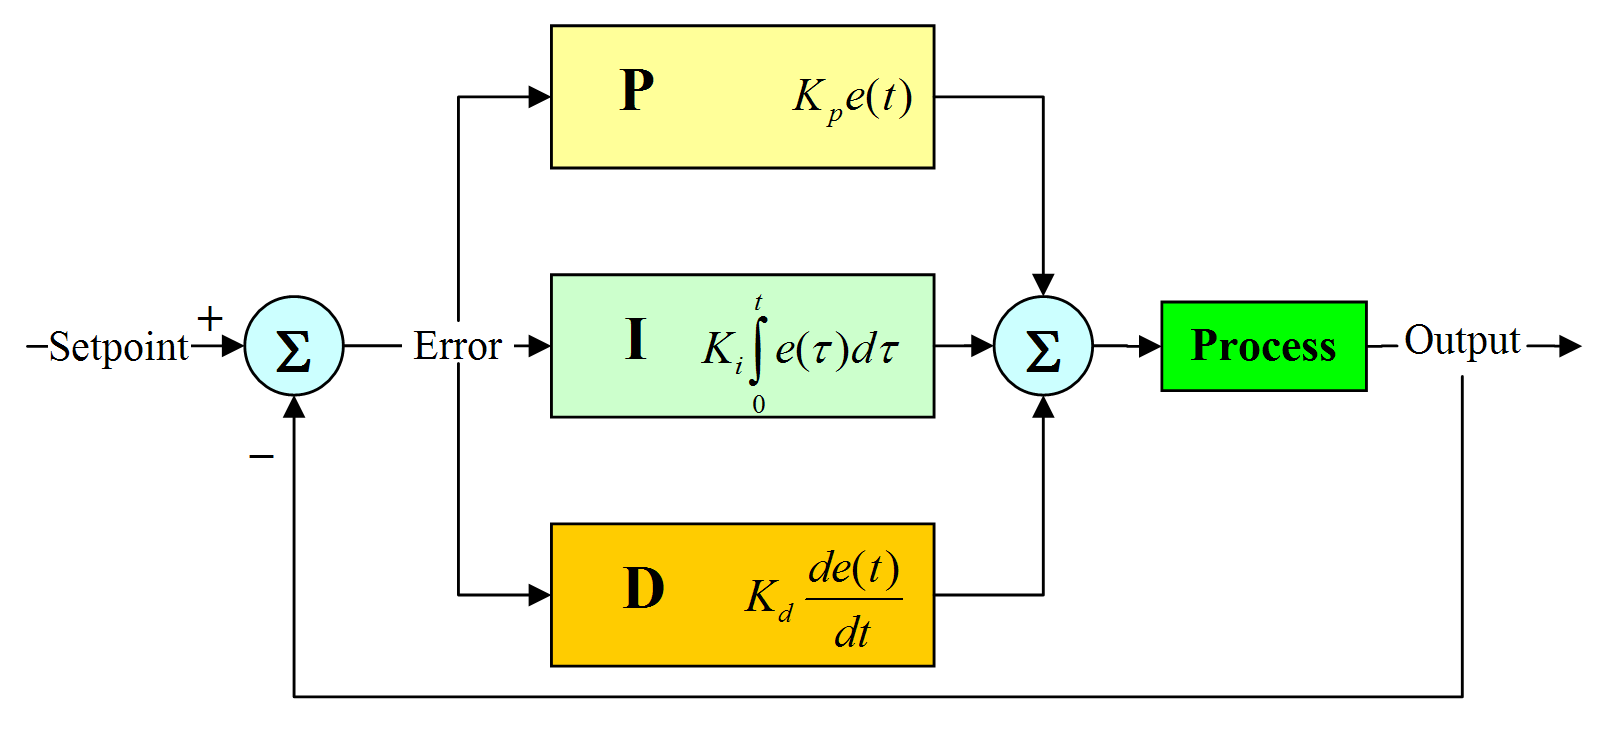
\includegraphics[width=0.8\textwidth]{../assets/images/motor-controllers/pid.png}
\caption{PID}
\end{figure}

Since \href{https://en.wikipedia.org/wiki/PID_controller}{PID} is an abbreviation, let's talk about that the terms $P$, $I$ and $D$ mean:
\begin{itemize}
\item $P$ stands for \textbf{proportional} -- how large is the error now (in the \textbf{present}).
\item $I$ stands for \textbf{integral} -- how large the error was in the \textbf{past.}
\item $D$ stands for \textbf{derivative} -- what will the error likely be in the \textbf{future.}
\end{itemize}\vspace{\parskip}

The controller takes into account what happened, what is happening, and what will likely happen, and combine these things to produce the controller value.


\subsubsection{Deriving the equations}
Before diving into the equations, we need to define a terms to build the equations from:
\begin{itemize}
\item $e$ -- the current error (difference between robot position and its goal).
\item $\Delta e$ -- difference between the current and the previous error.
\item $\Delta t$ -- time elapsed since the last measurement.
\item $p, i, d$ -- constants (positive real numbers) to determine, how important each of the terms are. This make it so that we can put more emphasis on some parts of the controller than others (or ignore them entirely).
\end{itemize}\vspace{\parskip}


\subsubsubsection{Proportional}
Proportional is quite straight forward -- it only takes into account, how big the error is right now.

\vspace{-\parskip}\[P = e\]

The problem with only using only $P$ is that the closer we get to the goal, the smaller the value of this term is. The robot's movement would feel stiff and there is a chance that it wouldn't even reach the goal. That's why it needs to be complemented by the other parts, for the controller to be effective.


\subsubsubsection{Integral}
Integral adds the extra push that the proportional was missing, because it doesn't react to what is happening right now, but to what was happening in the past, by accumulating the error.

\begin{figure}[H]
\centering
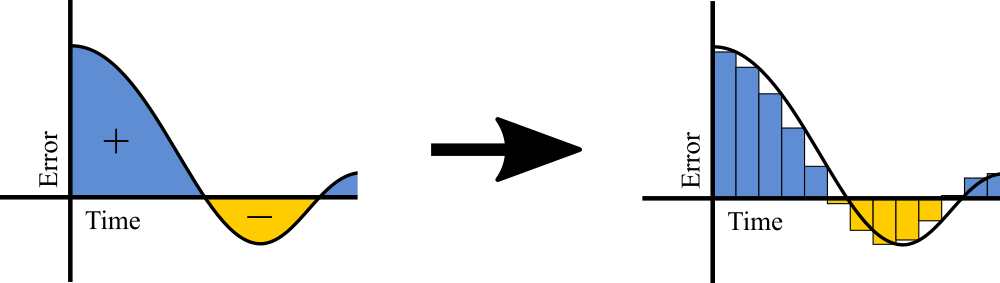
\includegraphics[width=0.8\textwidth]{../assets/images/motor-controllers/integral.png}
\caption{Integral}
\end{figure}

Calculating an \href{https://en.wikipedia.org/wiki/Integral}{integral} means calculating area under a curve (in our case, the curve is error over time). With real-world measurements, we can't calculate the actual area, because we can only call the code so many times a second. That's why we will approximate the area by calculating rectangles that closely resemble the curve.

For each computation, the height of the rectangle is the error $e$, and width is the elapsed time $\Delta t$ since the last measurement. To calculate the rectangular area, we multiply these two numbers together. $I$ itself is the sum of all of these values.

\vspace{-\parskip}\[I \mathrel{+}= e \cdot \Delta t\]

This can, however, introduce additional instability to the controller, since the values can accumulate and cause overshoot, and the reaction could also potentially be slow, due to \href{https://en.wikipedia.org/wiki/Integral_windup}{windup}.


\subsubsubsection{Derivative}
Derivative aims to further improve the controller by damping the values. We will calculate the rate of change of the error to predict its future behavior -- the faster the robot goes, the bigger $\Delta e$ is, and the more it will push back against the other terms.

\vspace{-\parskip}\[D = \frac{\Delta e}{\Delta t}\]

A note to be made is that if $\Delta t = 0$, the derivative can't be calculated, because we would be dividing by zero -- just something to keep in mind for the implementation.


\subsubsubsection{Result}
As we have previously said, the result is adding all of those terms, multiplied by their constants (determines the importance of the terms in the result).

\vspace{-\parskip}\[P \cdot p + I \cdot i + D \cdot d\]

The only thing we need to keep in mind is that the values could exceed $1$ (or $-1$). If they do, we will simply return $1$ (or $-1$).


\subsubsection{Implementation}
The controller will need the $p$, $i$ and $d$ constants. It will also need a feedback function and, to correctly calculate the integral and derivative, a function that returns the current time.

\begin{minted}{python}
class PID:
    """A class implementing a PID controller."""

    def __init__(self, p, i, d, get_current_time, get_feedback_value):
        """Initialises PID controller object from P, I, D constants, a function
        that returns current time and the feedback function."""
        # p, i, and d constants
        self.p, self.i, self.d = p, i, d

        # saves the functions that return the time and the feedback
        self.get_current_time = get_current_time
        self.get_feedback_value = get_feedback_value

    def reset(self):
        """Resets/creates variables for calculating the PID values."""
        # reset PID values
        self.proportional, self.integral, self.derivative = 0, 0, 0

        # reset previous time and error variables
        self.previous_time, self.previous_error = 0, 0

    def get_value(self):
        """Calculates and returns the PID value."""
        # calculate the error (how far off the goal are we)
        error = self.goal - self.get_feedback_value()

        # get current time
        time = self.get_current_time()

        # time and error differences to the previous get_value call
        delta_time = time - self.previous_time
        delta_error = error - self.previous_error

        # calculate proportional (just error times the p constant)
        self.proportional = self.p * error

        # calculate integral (error accumulated over time times the constant)
        self.integral += error * delta_time * self.i

        # calculate derivative (rate of change of the error)
        # for the rate of change, delta_time can't be 0 (divison by zero...)
        self.derivative = 0
        if delta_time > 0:
            self.derivative = delta_error / delta_time * self.d

        # update previous error and previous time values to the current values
        self.previous_time, self.previous_error = time, error

        # add P, I and D
        pid = self.proportional + self.integral + self.derivative

        # return pid adjusted to values from -1 to +1
        return 1 if pid > 1 else -1 if pid < -1 else pid

    def set_goal(self, goal):
        """Sets the goal and resets the controller variables."""
        self.goal = goal
        self.reset()
\end{minted}


To fully understand how the controller works, I suggest you closely examine the \texttt{get\_value()} function -- that's where all the computation happens.

Notice a new function called \texttt{reset} that we haven't seen in any of the other controllers. It is called every time we set the goal, because the controller accumulates error over time in the \texttt{integral} variable, and it would therefore take longer to adjust to the new goal.

It doesn't change the versatility of the controller classes, because we don't need to call it in order for the controller to function properly, it's just a useful function to have.


\subsubsection{Tuning the controller}
PID is the first discussed controller that needs to be tuned correctly to perform well (besides dead reckoning, where you have to correctly calculate the average speed). Tuning is done by adjusting the $p$, $i$ and $d$ constants, until the controller is performing the way we want it to.

There is a \href{https://en.wikipedia.org/wiki/PID_controller#Loop_tuning}{whole section} on Wikipedia about PID tuning. We won't go into details (read through the Wikipedia article if you're interested), but it is just something to keep in mind when using PID, because incorrect tuning could have \href{https://www.youtube.com/watch?v=MxALJU_hp34}{disastrous results}.


\subsubsection{Examples}

\subsubsubsection{Driving a distance}
Here is an example that makes the robot drive 10 meters forward. The constants are values that I used on the VEX EDR robot that I built to test the PID code, you will likely have to use different ones.

\begin{minted}{python}
# initialize objects that control robot components
left_motor = Motor(1)
right_motor = Motor(2)
encoder = Encoder()

# create a controller object and set its goal
controller = PID(0.07, 0.001, 0.002, time, encoder)
controller.set_goal(10)

while True:
    # get the controller value
    controller_value = controller.get_value()

    # drive the robot using tank drive controlled by the controller value
    tank_drive(controller_value, controller_value, left_motor, right_motor)
\end{minted}



\subsubsubsection{Auto-correct heading}
Auto-correcting the heading of a robot is something PID is great at. What we want is to program the robot so that if something (like an evil human) pushes it, the robot adjusts itself to head the way it was heading before the push.

We could either use values from the encoders on the left and the right side to calculate the angle, but a more accurate way is to use a gyroscope. Let's therefore assume that we have a \texttt{Gyro} class whose objects give us the current heading of the robot.

One thing we have to think about is what to set the motors to when we get the value from the controller, because to turn the robot, both of the motors will be going in opposite directions. Luckily, \texttt{arcade\_drive} is our savior -- we can plug our PID values directly into the turning part of arcade drive (the \texttt{x} axis) to steer the robot. Refer back to the Arcade Drive article, if you are unsure as to how/why this works.

\begin{minted}{python}
# initialize objects that control robot components
left_motor = Motor(1)
right_motor = Motor(2)
gyro = Gyro()

# create a controller object and set its goal
controller = PID(0.2, 0.002, 0.015, time, gyro)
controller.set_goal(0)  # the goal is 0 because we want to head straight

while True:
    # get the controller value
    controller_value = controller.get_value()

    # drive the robot using arcade drive controlled by the controller value
    arcade_drive(controller_value, 0, left_motor, right_motor)
\end{minted}



\subsubsection{Closing remarks}
PID is one of the most widely used controllers not just in robotics, but in many other industries, because it is reliable, relatively easy to implement and quite precise for most use cases.

For motivation, here is a \href{https://www.youtube.com/watch?v=4Y7zG48uHRo}{video} demonstrating the power of a correctly configured PID controller.





\subsection{Polynomial Function}
Another way that we can get values that aren't just 1's and 0's is to model a function from points and get the speed of the robot from it -- for example: let's say that we start at speed 0.2, drive at full speed when we're at half the distance and slow down to 0 when we're at the end.

Polynomial function is a great candidate for this task. We can pick points that we want the function to pass through and then use \href{https://en.wikipedia.org/wiki/Polynomial_regression}{polynomial regression} to get the coefficients of the function.

\begin{figure}[H]
\centering
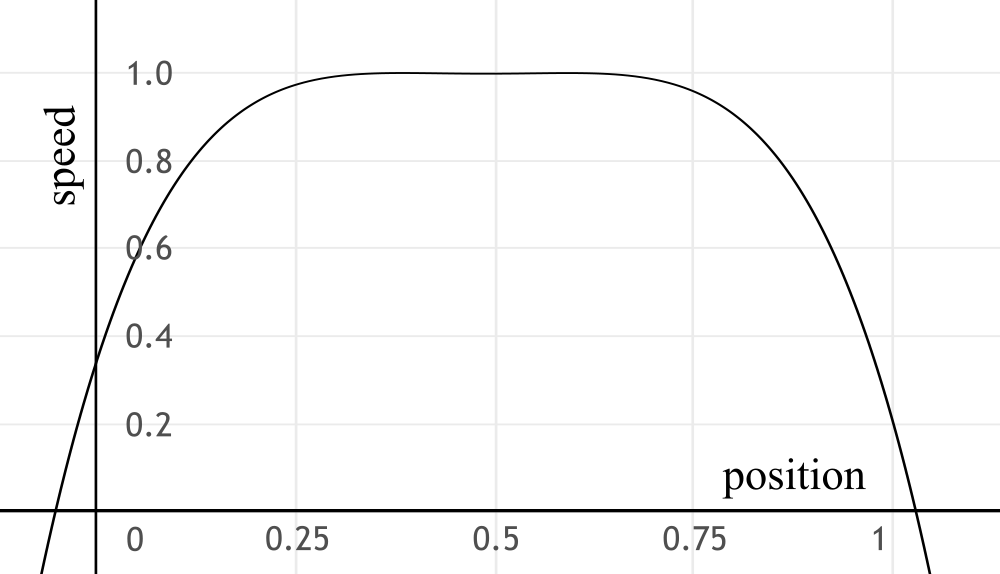
\includegraphics[width=0.8\textwidth]{../assets/images/motor-controllers/polynomial-function.png}
\caption{Polynomial function}
\end{figure}

One thing you should also notice is that the function starts at $x = 0$ and ends at $x = 1$. This is deliberate -- it makes it easy for us to "stretch" the function a little wider if we want to drive some other distance, not just a distance of 1.


\subsubsection{Horner's method}
When it comes to programming, exponentiation tends to be quite expensive. \href{https://en.wikipedia.org/wiki/Horner\%27s_method}{Horner's method} is an elegant solution to this problem. The concept is simple -- change the expression by repeatedly taking out $x$, so there is no exponentiation.

\vspace{-\parskip}\[2x^3 + 4x^2 -x + 5 \quad \rightarrow \quad x(x(x(2) + 4) - 1) + 5\]

This requires fewer multiplications, thus making the evaluation faster.


\subsubsection{Implementation}
The controller only needs the coefficients of the polynomial that we modeled, and a feedback function.

\begin{minted}{python}
class PolynomialFunction:
    """A class implementing a polynomial function controller."""

    def __init__(self, coefficients, get_feedback_value):
        """Initialises the polynomial function controller from the polynomial
        coefficients and the feedback value."""
        self.coefficients = coefficients    # the coefficients of the function
        self.get_feedback_value = get_feedback_value   # the feedback function

    def get_value(self):
        """Returns the polynomial function value at feedback function value."""
        # calculate the x coordinate (by "stretching" the function by goal)
        x = self.get_feedback_value() / abs(self.goal)

        # calculate function value using Horner's method
        value = self.coefficients[0]
        for i in range(1, len(self.coefficients)):
            value = x * value + self.coefficients[i]

        # if the value is over 1, set it to 1
        if value > 1:
            value = 1

        # if goal is negative, function value is negative
        return value if self.goal > 0 else -value

    def set_goal(self, goal):
        """Sets the goal of the controller."""
        self.goal = goal
\end{minted}



\subsubsection{Examples}

\subsubsubsection{Driving a distance}
Once again, the code is almost the exact same as the examples from nearly all of the other controllers.

\begin{minted}{python}
# initialize objects that control robot components
left_motor = Motor(1)
right_motor = Motor(2)
encoder = Encoder()

# create a controller object and set its goal
controller = PolynomialFunction([-15.69, 30.56, -21.97, 6.91, 0.2], encoder)
controller.set_goal(10)

while True:
    # get the controller value
    controller_value = controller.get_value()

    # drive the robot using tank drive controlled by the controller value
    tank_drive(controller_value, controller_value, left_motor, right_motor)
\end{minted}



\subsubsection{Generating a polynomial}
An alternative to "stretching" the polynomial to fit the goal is to specify the points the polynomial passes through and generate the coefficients \textit{after} the goal is specified.

Say you have points $\left(0,0.2\right)$, $\left(0.4,1\right)$, $\left(0.6,1\right)$ and $\left(1,0\right)$. Since there are 4 points, the general form of the polynomial is $y=ax^3+bx^2+cx+d$ Using this information, we can create a system of linear equations:

$$\begin{array}{rcl}
0.2 & = & a(0)^3+b(0)^2+c(0)+d \\
1   & = & a(0.4)^3+b(0.4)^2+c(0.4)+d \\
1   & = & a(0.6)^3+b(0.6)^2+c(0.6)+d \\
0   & = & a(1)^3+b(1)^2+c(1)+d
\end{array}$$

Solving this system of linear equations will give us the coefficients of the polynomial. We can apply this method to a polynomial of any degree $d$, if we have at least $d+1$ number of points.


\subsubsection{Closing remarks}
Although this controller isn't as widely used as PID, it can sometimes outperform PID, namely in situations where the ranges of movement of the motors are restricted -- forks of a forklift/robot arm.




\section{Odometry}





Odometry is the use of data from sensors of the robot to estimate its position over time.

This means that we can calculate where the robot is at the moment, by getting information from sensors such as an encoder, a gyro, or a camera, and performing calculations on said information.




\subsection{Heading from Encoders}
There are two things we need to know to approximate the position:
\begin{itemize}
\item \textbf{Distance $\Delta$} -- how much did we move by?
\item \textbf{Heading $\Delta$} -- which way are we heading?
\end{itemize}\vspace{\parskip}

Assuming we have encoders on both sides of the robot, the distance is easy to calculate: we can read the values the encoders on both of the sides are reading and average them. Assuming we also have a gyro, heading is easy too: we can get the heading directly as the values the gyro is returning.

But what if we didn't have a gyro?


\subsubsection{Calculate heading without gyro}
Although gyro is arguably the most precise way to measure the current heading, it's not always available. It might be too expensive, impractical to include on a small robot, or not viable because of other conditions. In cases like these, it is good to know how to calculate heading only from the encoders.

Say the robot drove a small arc. The left encoder measured a distance $l$ and the right side measured a distance $r$. The length between the two wheels of the drivetrain is $c$, the angle by which we turned is $\omega$ (measured in radians), and $x$ is just a variable to help with our calculations.

\begin{figure}[H]
\centering
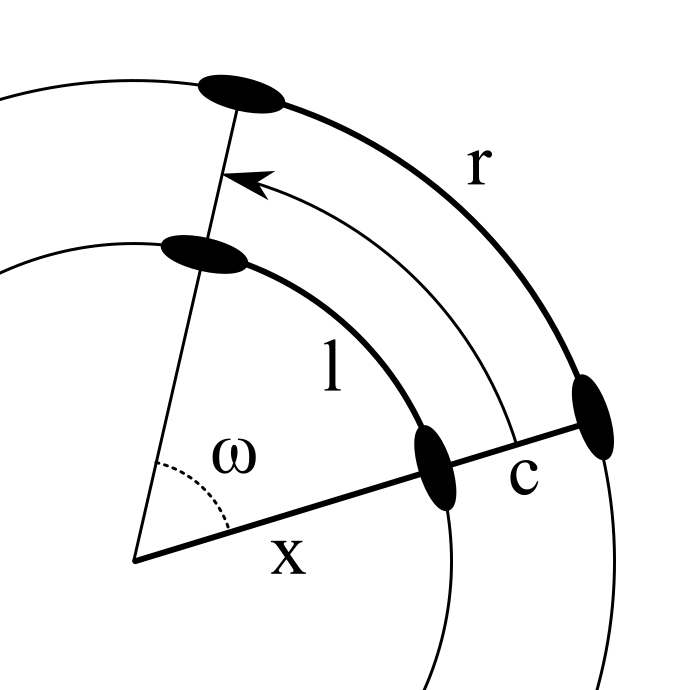
\includegraphics[width=0.8\textwidth]{../assets/images/odometry/heading-from-encoders.png}
\caption{Heading from encoders}
\end{figure}

Let's derive the equations for the lengths of the arches $l$ and $r$ in terms of the other variables (here is an article about \href{https://www.mathopenref.com/arclength.html}{arc length}, if you need further clarification):

\vspace{-\parskip}\[l=x\cdot\omega\qquad r=\left(c+x\right)\cdot\omega\]

We can then combine the equations, simplify, and solve for $\omega$:

\vspace{-\parskip}\[\frac{l}{\omega} = \frac{r}{\omega} - c\]

\vspace{-\parskip}\[\omega = \frac{r - l}{c}\]

And that's it! The angle can be calculated from the difference of the readings of the encoders, divided by the length of the axis.





\subsection{Line Approximation}
For our first approximation, let's make an assumption: instead of driving an arc, the robot will first turn by the specified angle, and only then drive the distance in a straight line.

This is quite a reasonable assumption to make for smaller angles: since we are updating the position multiple times per second, the angles aren't going to be too large.

\begin{figure}[H]
\centering
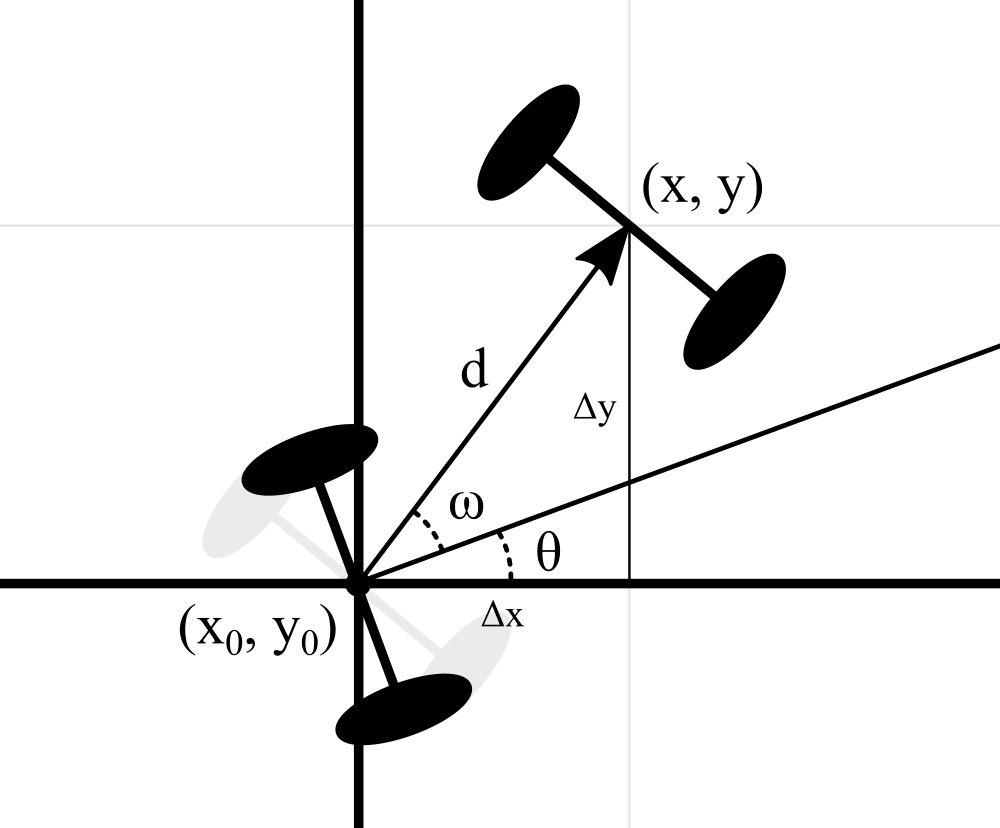
\includegraphics[width=0.8\textwidth]{../assets/images/odometry/line-approximation.png}
\caption{Line Approximation}
\end{figure}

\subsubsection{Deriving the equations}
The robot moved a distance $d$. It was previously at an angle $\theta$ and is now at an angle $\theta + \omega$. We want to calculate, what the new position of the robot is after this move.

One of the ways to do this is to imagine a right triangle with $d$ being hypotenuse. We will use \href{https://www2.clarku.edu/faculty/djoyce/trig/formulas.html}{trigonometric formulas} and solve for $\Delta x$ and $\Delta y$:

\vspace{-\parskip}\[sin(\theta + \omega)=\frac{\Delta y}{d} \qquad cos(\theta + \omega)=\frac{\Delta x}{d}\]

\vspace{-\parskip}\[\Delta y = d \cdot sin(\theta + \omega) \qquad \Delta x = d \cdot cos(\theta + \omega)\]

The resulting coordinates $(x,y)$ are $x=x_0+\Delta x$ and $y=y_0+\Delta y$.


\subsubsection{Implementation}
This is one of the possible implementations of a class that tracks the current position of the robot by getting information from both encoders using the aforementioned line approximation method.

Note that for the position estimation to be accurate, the \texttt{update()} function of the class needs to be called multiple times per second.

\begin{minted}{python}
from math import cos, sin


class LineApproximation:
    """A class to track the position of the robot in a system of coordinates
    using only encoders as feedback, using the line approximation method."""

    def __init__(self, axis_width, l_encoder, r_encoder):
        """Saves input values, initializes class variables."""
        self.axis_width = axis_width
        self.l_encoder,  self.r_encoder = l_encoder, r_encoder

        # previous values for the encoder position and heading
        self.prev_l, self.prev_r, self.prev_heading = 0, 0, 0

        # starting position of the robot
        self.x, self.y = 0, 0

    def update(self):
        """Update the position of the robot."""
        # get sensor values and the previous heading
        l, r, heading = self.l_encoder(), self.r_encoder(), self.prev_heading

        # calculate encoder deltas (differences from this and previous readings)
        l_delta, r_delta = l - self.prev_l, r - self.prev_r

        # calculate omega
        h_delta = (r_delta - l_delta) / self.axis_width

        # approximate the position using the line approximation method
        self.x += l_delta * cos(heading + h_delta)
        self.y += r_delta * sin(heading + h_delta)

        # set previous values to current values
        self.prev_l, self.prev_r, self.prev_heading = l, r, heading + h_delta

    def get_position(self):
        """Return the position of the robot."""
        return (self.x, self.y)
\end{minted}






\subsection{Circle Approximation}
Although the line approximation is relatively accurate, we can make it more precise by assuming that the robot drives in an arc, which, in reality, is closer to what the robot is really doing.

\begin{figure}[H]
\centering

\includegraphics[width=0.8\textwidth]{../assets/images/odometry/circle-approximation.png}
\caption{Circle Approximation}
\end{figure}

\subsubsection{Deriving the equations}
The robot moved in an arch, the left encoder measured a distance $l$ and the right wheel a distance $r$. It was previously at an angle $\theta$ and is now at an angle $\theta + \omega$. We want to calculate, what the new position of the robot is after this move.

The way to calculate the new coordinates is to find the radius $R$ of \href{https://en.wikipedia.org/wiki/Instant_centre_of_rotation}{ICC} (\textit{Instantaneous Center of Curvature} -- the point around which the robot is turning) and then rotate $x_0$ and $y_0$ around it.


\subsubsubsection{Calculating R}
Let's start by finding the formula for calculating $R$. We will derive it from the formulas for calculating $l$ and $r$:

\vspace{-\parskip}\[l = \omega \cdot \left(R - \frac{c}{2}\right) \qquad r = \omega \cdot \left(R + \frac{c}{2}\right)\]

Combining the equations and solving for R gives us:

\vspace{-\parskip}\[R = \left(\frac{r+l}{\omega \cdot 2} \right)\]

From our previous article about Heading from Encoders, we know that $\omega = \frac{r - l}{c}$. If we don't have a gyro, we can just plug that into our newly derived formula and get:

\vspace{-\parskip}\[R = \frac{r+l}{\frac{r - l}{c} \cdot 2} = \frac{r+l}{r - l} \cdot \frac{c}{2}\]


\subsubsubsection{Rotating $(x_0, y_0)$ around ICC}
For this section, we will assume that you know how to rotate a point around the origin by a certain angle. If not, here is a \href{https://www.khanacademy.org/partner-content/pixar/sets/rotation/v/sets-8}{video} from Khan Academy deriving the equations.

First of, we will need the coordinates of the $ICC$. Since it's perpendicular to the left of the robot, we can calculate it by first calculating a point that is distance $R$ in front of the robot:

\vspace{-\parskip}\[ICC_x=x_0+R \; cos(\theta) \qquad ICC_y=y_0+R \cdot sin(\theta)\]

We will then turn the point 90 degrees to place it at distance $R$ perpendicular to the robot by switching $x_0$ and $y_0$ and negating the first coordinate (using \href{https://stackoverflow.com/questions/4780119/2d-euclidean-vector-rotations}{simple vector algebra}):

\vspace{-\parskip}\[ICC_x=x_0-R \; sin(\theta) \qquad ICC_y=y_0+R \cdot cos(\theta)\]

To rotate $(x_0, y_0)$ around ICC (and therefore find $(x, y)$), we will first translate ICC to the origin, then rotate, and then translate back:

\vspace{-\parskip}\[x = (x_0 - ICC_x) \cdot cos(\omega) - (y_0 - ICC_y) \cdot sin(\omega) + ICC_x\]

\vspace{-\parskip}\[y = (x_0 - ICC_x) \cdot sin(\omega) + (y_0 - ICC_y) \cdot cos(\omega) + ICC_y\]

Plugging in the values for $ICC_x$, $ICC_y$ and simplifying:

\vspace{-\parskip}\[x = R \; sin(\theta) \cdot cos(\omega) + R \cdot cos(\theta) \cdot sin(\omega) + x_0 - R \; sin(\theta)\]

\vspace{-\parskip}\[y = R \; sin(\theta) \cdot sin(\omega) - R \cdot cos(\theta) \cdot cos(\omega) + y_0 + R \; cos(\theta)\]

Using trigonometric rules, the equations can be further simplified to:

\vspace{-\parskip}\[x = x_0 + R \; sin(\theta + \omega) - R \; sin(\theta)\]

\vspace{-\parskip}\[y = y_0 - R \; cos(\theta + \omega) + R \; cos(\theta)\]


\subsubsubsection{Edge cases}
There is one noteworthy case of values $l$ and $r$ where our circle approximation method won't work.

If $r=l$ (if we are driving straight), then the radius cannot be calculated, because it would be "infinite". For this reason, our method can't be used on its own, because if the robot drove in a straight line, the code would crash.

We can, however, still employ or line approximation method, since in this case, it really is driving in a straight line! It is also a good idea to apply the line approximation method for very small angles, since it's almost like driving straight, and it's less computationally intensive to the circle approximation method.


\subsubsection{Implementation}
Here is the implementation, combining both of the approximation methods:

\begin{minted}{python}
from math import cos, sin


class CircleApproximation:
    """A class to track the position of the robot in a system of coordinates
    using only encoders as feedback, using a combination of line and circle
    approximation methods."""

    def __init__(self, axis_width, l_encoder, r_encoder):
        """Saves input values, initializes class variables."""
        self.axis_width = axis_width
        self.l_encoder,  self.r_encoder = l_encoder, r_encoder

        # previous values for the encoder position and heading
        self.prev_l, self.prev_r, self.prev_heading = 0, 0, 0

        # starting position of the robot
        self.x, self.y = 0, 0

    def update(self):
        """Update the position of the robot."""
        # get sensor values and the previous heading
        l, r, heading = self.l_encoder(), self.r_encoder(), self.prev_heading

        # calculate encoder deltas (differences from this and previous readings)
        l_delta, r_delta = l - self.prev_l, r - self.prev_r

        # calculate omega
        h_delta = (r_delta - l_delta) / self.axis_width

        # either approximate if we're going (almost) straight or calculate arc
        if abs(l_delta - r_delta) < 1e-5:
            self.x += l_delta * cos(heading)
            self.y += r_delta * sin(heading)
        else:
            # calculate the radius of ICC
            R = (self.axis_width / 2) * (r_delta + l_delta) / (r_delta - l_delta)

            # calculate the robot position by finding a point that is rotated
            # around ICC by heading delta
            self.x += R * sin(h_delta + heading) - R * sin(heading)
            self.y += - R * cos(h_delta + heading) + R * cos(heading)

        # set previous values to current values
        self.prev_l, self.prev_r, self.prev_heading = l, r, heading + h_delta

    def get_position(self):
        """Return the position of the robot."""
        return (self.x, self.y)
\end{minted}





\section{Resources}


Links to resources either directly used by the website (such as libraries), or those that helped me understand the concepts mentioned in the articles.


\subsection{Math}
The website uses \href{https://katex.org/}{$\text{\KaTeX}$} to render $\text{\LaTeX}$ equations.

\subsection{Images}
The images used to illustrate the concepts on this website are modified using \href{https://inkscape.org/cs/}{Inkscape} (free vector graphics editor) and \href{https://www.gimp.org/}{GIMP} (free bitmap graphics editor). CAD model images are generated with \href{https://www.autodesk.com/products/fusion-360/students-teachers-educators}{Fusion 360} (free CAD design software, assuming you are a student). I also used the \href{https://tinypng.com/}{TinyPNG} website to compress the images.

\subsection{p5.js}
Visualizations on the website are created using the \href{https://p5js.org/}{p5.js} library. This \href{https://raw.githubusercontent.com/KevinWorkman/HappyCoding/gh-pages/examples/p5js/_posts/2018-07-04-fireworks.md}{example} helped me understand how it worked with Jekyll. I use the \href{https://editor.p5js.org/}{p5js web editor} to edit the visualizations before I put them on the website.

\subsection{VEX EDR}
To test the algorithms, I built a custom VEX EDR robot using \href{https://www.vexrobotics.com/276-3000.html}{this kit} that the educational center \href{http://www.vctu.cz/}{VCT} kindly lent me. The robot is programed in Python using \href{https://www.robotmesh.com/studio}{RobotMesh studio} (for more information, see the Python \href{https://www.robotmesh.com/docs/vexcortex-python/html/namespaces.html}{documentation}).

\subsection{Autonomous motion control}
\href{https://github.com/AtsushiSakai/PythonRobotics}{PythonRobotics} is a great repository containing implementations of various robotics algorithms in Python.

\subsection{PID}
I studied a PID Python \href{https://github.com/ivmech/ivPID}{implementation} before writing my own.

\subsection{Drivetrain Control}
There were a few helpful articles that helped me understand equations behind the more complex drivetrains:
\begin{itemize}
\item Arcade drive Chief Delphi forum \href{https://www.chiefdelphi.com/media/papers/2661}{post} by Ether.
\item Simplistic Control of Mecanum Drive \href{https://forums.parallax.com/discussion/download/79828/ControllingMecanumDrive\%255B1\%255D.pdf&sa=U&ved=0ahUKEwiX5LzFiNrfAhVswYsKHTofDrwQFggEMAA&client=internal-uds-cse&cx=002870150170079142498:hq1zjyfbawy&usg=AOvVaw19D74YD--M3YmQ2MGd1rTg}{paper}.
\item Swerve drive Chief Delphi forum \href{https://www.chiefdelphi.com/t/paper-4-wheel-independent-drive-independent-steering-swerve/107383}{post} by Ether.
\end{itemize}\vspace{\parskip}

\subsection{Circle Approximation}
There were two main resources that helped me write the Circle Approximation article.
\begin{itemize}
\item Kinematics Equations for Differential Drive and Articulated Steering \href{http://www8.cs.umu.se/kurser/5DV122/HT13/material/Hellstrom-ForwardKinematics.pdf}{whitepaper}
\item Position Estimation \href{http://people.scs.carleton.ca/~lanthier/teaching/COMP4807/Notes/5\%20-\%20PositionEstimation.pdf}{presentation}
\end{itemize}\vspace{\parskip}





\section{About}





\subsection{Motivation}
When I joined the FRC team \href{https://www.metalmoose.org/}{Metal Moose} and started learning about robotics, I didn't find many beginner-friendly resources for people like me. They were hard to find and scattered all around the web. One had to be quite persistent to actually learn something on their own.

That is the main reason for the creation of this website -- to serve as a resource for people that want to learn the concepts of robotics, without having to go though all the trouble of finding quality resources.


\subsection{Contributions}
I accept any and all recommendations/suggestions about this website. If there is anything you think should be changed/corrected, or you have a topic that you wish there was an article about, feel free to let me know.

You can do so either by email (\texttt{tomas.slama.131@gmail.com}), or by creating an issue on the website's GitHub repositories (see link on the top right of this page).


\subsection{Acknowledgements}
I would like to thank the following people for their help in making this project a reality:
\begin{itemize}
\item \textbf{Ing. Daniel Kajzr} for insightful conversations about the project.
\item \textbf{Kateřina Sulková} for being loving, supportive, and especially helpful in writing the SOČ paper.
\item \textbf{Matěj Halama} (\textit{matejhalama.cz}) and \textbf{Jan Hladík} for help in designing the logo of the website.
\item \textbf{VCT} for kindly lending me a VEX EDR kit to work with.
\end{itemize}\vspace{\parskip}



\end{document}
